\documentclass[12pt,a4paper,bibtotoc,pointlessnumbers]{scrartcl}
\usepackage[ngerman]{babel}
%\usepackage[german]{polyglossia}
%\selectlanguage{german}
% ##########################################
% PDFLaTeX oder nicht:
\newif \ifPDF                                   
\ifx \pdfoutput \undifined \PDFfalse 
\else \ifnum \pdfoutput >0 \PDFtrue
     \else \PDFfalse         
     \fi     
\fi 
% ##########################################
\usepackage{lmodern} %ersetzt Standarsschrift --> für schönere Textdarstellung im PDF
\usepackage[onehalfspacing]{setspace} %setzt das Dokument in 1,5-fachem Zeilenabstand
\setlength\parindent{0pt}% Setzt den Einzug nach einem Absatz fest (hier auf Null)
\usepackage{microtype}

%\usepackage{csquotes}
%\usepackage[style=acm]{biblatex}
%\addbibresource{Literaur.bib}
\usepackage{bibgerm}
%\usepackage{natbib}

\usepackage[
backend=biber,
style=numeric,
%-verb
sorting=none
]{biblatex}
\addbibresource{BA-JannesBrunner.bib}
%\addbibresource{Bildquellen.bib}
%%\bibliography{Masterarbeit.bib}
%\usepackage{cite}


\usepackage[T1]{fontenc} %für europäischen ASCII-Code (mit Umlauten etc)
\usepackage[utf8]{inputenc} %Legt den Zeichencode fest

\usepackage[babel, german=quotes]{csquotes}

\usepackage[dvips]{graphicx} %damit Bilder eingebunden werden Können
\usepackage{fancyhdr} %Nachfolger zu "fancyheadings" --> legt Layout der Seite fest + hält zusätzliche Befehle und Optionen bereit

%\usepackage[headsepline]{scrlayer-scrpage}
%\automark[section]{subsection}

\usepackage{float} %Objekte, die nicht auf zwei Seiten aufgeteilt werden sollen (z.B. Bilder, Tabellen)
\usepackage{floatflt} %wird für die Umgebung floatfigure benötigt --> Bild kann von text umflossen werden
\usepackage[section]{placeins} %section verhindert, dass Bilder aus section hinausgleiten

\usepackage{amsmath} %für Matheumgebung
\usepackage{amssymb} %Setzt Befehle für Symbole in Symbole um 
\usepackage{amsfonts} %Zusätzliche Schriften und Symbole
\usepackage{exscale} %stellt Befehle für Änderung der Schrift bereit
\usepackage{textcomp}
\usepackage{easymat} % weitere Befehle für Matrizen
\usepackage{enumitem} % Ändern von Listenumgebungen
%\usepackage{paralist}

\usepackage{pdfpages}%erlaubt das einbinden von anderen PDF-Dokumenten (auch einzelnen Seiten) in das Latex-Dokument

\usepackage{etex} %erhöht die Anzahl der Pakete, die geladen werden können

\usepackage[font=small,labelfont=bf,hang]{caption} %für Bild- und Tabellenunterschriften
\addto\captionsngerman
{
	\renewcommand{\figurename}{\small{\textbf{Abb.}}}
	\captionsetup{figurewithin = section}
}
\addto\captionsngerman{
	\renewcommand{\tablename}{\small{Tab.}}}
\captionsetup{tablewithin = section}
\captionsetup{font=small, labelfont=bf}

%\usepackage{subfig}
\usepackage{subcaption}
\usepackage{longtable}% erlaubt Tabellen über mehrere Seiten
\usepackage{tabularx} %Tabellen können größer gemacht werden und und die Spalten sind flexibler
\usepackage{booktabs} %definiert Befehle für Tabellen
%\usepackage{booktabs-de}
\usepackage{ltxtable} %vereinigt longtable und tabularx
\usepackage{colortbl}
\usepackage{multirow}
%\usepackage{multicolumn}
\usepackage{rotating}
%\usepackage{tablefootnote}

%\usepackage{tikz}

\usepackage{array} %erweiterte Möglichkeiten für Tabellen und Spalten
%\usepackage{subfigure}
\usepackage{url} %lange Zeichenfolgen können trotz fehlender Leerzeichen getrennt werden
%\usepackage{paralist}
% ##########################################

% ##########################################
% Seitendesign:
\usepackage{units}
\usepackage[headheight=50pt, a4paper, bottom=25mm, footskip=6mm]{geometry} %wird für Layout des Dokuments benötigt
\geometry{verbose}
% ##########################################
%\usepackage{cite} % fasst Zitate zusammen (funktioniert nur ohne hyperref)

\ifPDF
\usepackage{xcolor}   %ermöglicht das Ändern der Farbe von Schrift, Seitenhintergrund, Boxen etc
\usepackage[
  pdftex,
  colorlinks,
  citecolor = {green},
  linkcolor = {black},
  urlcolor  = {gray},                
  bookmarks         = true,
  bookmarksopen     = true, % Bookmarks anzeigen...
  bookmarksnumbered = true, % ...und numerieren
  pdftitle          = {Masterarbeit},
  pdfauthor         = {Nanin Brunner}
]{hyperref} %ermöglicht Links im PDF-Dokument (z.B. ancklicken eines Kapitel im Inhaltsverzeichnis oder Verlinkung mit externem Link)


\else
\usepackage{wrapfig}
%\usepackage{floatflt} %ermöglicht Gleitobjekte (Bilder, Tabellen) von Text umfließen zu lassen und Bilder links/recht je nach Seitenzahl auszurichten
\fi%-----------------------------------------------------------------------------
% Definition für einen neuen Befehl für deutsche Anführungszeichen
\newcommand{\gqq}[1]{\glqq{}#1\grqq{}}
\newcommand{\gq}[1]{\glq{}#1\grq{}}


\begin{document}
	\begin{titlepage}
		\begin{center}
%				\begin{figure}[h]
%					\begin{minipage}{.4\textwidth}
%						\centering
%						\includegraphics[width=0.5\textwidth]{Bilder/Logo_Wildau}
%					\end{minipage}
%					\begin{minipage}{.2\textwidth}
%						\hspace{\textwidth}
%					\end{minipage}
%					\begin{minipage}{.4\textwidth}
%						\centering
%						\includegraphics[width=0.4\textwidth]{Bilder/bam_logo_135}
%					\end{minipage}
%				\end{figure}			
%				\vspace{0.4cm}
			
%			{\large \bf Bundesanstalt für Materialforschung und -prüfung }\\[4mm]
%			{\large\bf TH Wildau}
			%\vspace{0.5cm} \hrule \vspace{1.3cm}
			
			 
			\begin{doublespace}
			{\huge Entwicklung einer webbasierten Client-Server Anwendung zur Unterstützung von interaktiven Unterrichtsmethoden}\\
			\end{doublespace}
			\vspace{2cm}
			
			{\huge \bf Bachelorarbeit}\\
			\vspace{0.4cm}
			
			{\large zur Erlangung des akademischen Grades\\ Bachelor\\ (B.-Sc.)\\an der HTW Berlin}\\
			
			\vspace{1cm}
			
			{\Large \bf Hochschule für Technik und Wirtschaft Berlin}\\
			{\large \bf Fachbereich Informatik, Kommunikation und Wirtschaft\\
			Studiengang internationale Medieninformatik}\\
		
			\vspace{1.5cm}
			
			{\doublespacing Eingereicht von\\
			{\Large \bf Jannes Julian Brunner}\\ geb. 21.06.1991}
			
%			\vspace{1cm}
		
			\large
			\begin{table}[b]
				\begin{center}
					\begin{tabular}{ll}
					Eingereicht am:& 29.07.2019\\
					Betreuender Hochschuldozent:& Prof. Dr. Gefei Zhang\\
					Zweitgutachter: & Prof. Dr.-Ing. Kai Uwe Barthel\\
					\end{tabular}
				\end{center}
			\end{table} 
		\end{center}
		\vspace{0.6cm}
	%	{\bf Abstract}: Das Abstract
\end{titlepage}

\newpage
%\clearpairofpagestyles




%\clearpairofpagestyles

\pagenumbering{roman}
\setcounter{page}{10}

\section*{Abstract}\label{sec:abstract}
\newpage

%\thispagestyle{empty}
\cfoot{\pagemark}
\tableofcontents 
\newpage

\pagenumbering{arabic}




%\pagestyle{scrheadings}
%\ihead{\leftmark}
%%\automark{section}
%\chead{\rightmark}
%%\automark{subsection}
%\ohead{\thepage}


\pagestyle{fancy}
\fancyhf{}
%\setlength{\headheight}{15pt}
\renewcommand{\headrulewidth}{0.4pt} %definiert die Dicke der Linie unter der Kopfzeile
%\renewcommand{\footrulewidth}{0pt} %definiert die Dicke der Linie über der Fußzeile
\renewcommand{\sectionmark}[1]{%
	\markboth{\thesection.\ #1}{}} %sorgt dafüpr, dass die Kapitel und Unterkapitel in der Kopfzeile stehen


%\addtolength{\headwidth}{\marginparwidth}
%\setlength{\fancyhead}{0.4\headrulewidth}
\fancyhead[L]{\textsl{\small 
%		\leftmark \hspace{0.8cm}
		\rightmark}}
%\fancyhead[C]{\parbox{0.5\textwidth}{\textsl{\small \rightmark}}}
\fancyhead[R]{\textsl{\small \thepage}}
%\fancyhead[L]{\parbox{0.3\textwidth}{\textsl{\small \leftmark}}}
%\fancyhead[C]{\parbox{0.6\textwidth}{\textsl{\small \rightmark}}}
%\fancyhead[R]{\parbox{0.05\textwidth}{\textsl{\small \thepage}}}
%\addtolength{\headwidth}{\marginparsep}
%\fancyfoot[C]{\thepage}


\thispagestyle{empty}
\section*{Selbstständigkeitserklärung}\label{sec:selbststandigkeitserklarung}
Ich erkläre hiermit, dass ich die vorliegende Bachelorarbeit selbstständig verfasst und dazu  keine  anderen  als  die  angeführten  Behelfe  verwendet,  die  Autorenschaft  eines Textes  nicht  angemaßt  und  wissenschaftliche  Texte  oder  Daten  nicht  unbefugt verwertet habe. Die elektronische Kopie ist mit den gedruckten Exemplaren identisch.
\vspace{5cm}
\\

Berlin, \today, 
\begin{flushleft}
	\line(1,0){350}\\
	(Ort, Datum, Unterschrift)
\end{flushleft}
\newpage

\section{Einführung}\label{sec:einfuhrung}
\subsection{Motivation}\label{sec:motivation}

Bildung ist ein wichtiges Element der Persönlichkeitsentwicklung und unter Artikel 26 der allgemeinen Erklärung der Menschenrechte als solches definiert. Ohne Bildung ist das Ausüben eines gewählten Berufes und das Entwickeln einer Meinung zu komplexen Sachverhalten unmöglich. \cite{weitblicker.org2019:online}. Heute sieht sich Bildung durch den digitalen Wandel der letzten Jahre sich noch nie vorher dagewesenen Problemen gegenübergestellt. Wie können Lehrende an Schulen digitale Technik effizient und preiswert im Unterricht einsetzen und so neue Bildungskonzepte erfolgreich in den Lehrplan integrieren? Ursprünglich bezeichnet der Begriff Digitalisierung das Umwandeln von Analog nach Digital. Wurde früher Musik auf Schallplatten vertrieben, so wurde diese von der Compact Disc vom Markt verdrängt, welche die Musik auf kleinerem Raum digital abspeichert. Auch wenn der Begriff im Zusammenhang mit Schule längst nicht mehr das Ursprüngliche meint, halte ich es für sehr wichtig, früher dagewesene Unterrichtskonzepte nicht einfach zu digitalisieren sondern es erfordert ein Neudenken. Bewährte pädagogische Methoden sollten durch Digitalisierung profitieren sowie neue Konzepte müssen erforscht und entwickelt werden. 

\subsubsection{Besuch Grundschule am Rüdesheimer Platz Berlin}\label{sec:grundschulebesuch}
Im Rahmen der Vorrecherche zu dieser Arbeit wurde einem Unterrichtstag in 
einer Jahrgangsübergreifenden (JüL) Klasse 1 bis 3 an der Grundschule am Rüdesheimer Platz beigewohnt um ein differenzierteres 
Bild der gegenwärtigen Lern- und Digitalisierungssituation an einer Berliner Schule zu bekommen. An dieser Stelle eine große Dankaussagung an Frau Wewer, Grundschullehrerin, welche diese Erfahrung möglich gemacht hat und in einem anschließenden Gespräch das Interesse an einer kostengünstigen und einfach nutzbaren Lösung zur Unterstützung von interaktiven Unterrichtsmethoden unterstrichen hat.
\newpage
\subsection{Problemstellung}\label{sec:problemstellung}
%Kurze Zusammenfassung des Forschungsstandes genügend?
Am 04.04.2019 trat die Änderung des Art. 104c des Grundgesetz für die Bundesrepublik Deutschland in Kraft
und ebnete so den Weg für den von Bund und Ländern beschlossenen Digitalpakt Schule \cite{Art104cG55:online}. 
Dieser Beschluss macht deutlich, dass digitale Kompetenz im Bildungssektor von hoher Bedeutung ist, was auch von einer Förderungssumme von mindestens 5,5 Milliarden Euro unterstrichen wird. 
Legt man diese Summe auf die ca 40.000 Schulen um, erhält jede Schule einen Durchschnittsbeitrag von 137.000 Euro. Bei ca. 11 Millionen Schülerinnen und Schülern würde das eine Förderungssumme von ca. 500 Euro pro Schülerin bzw. Schüler bedeuten. 
Einer der Hauptförderungspunkte des Digitalpakt Schule sieht den Ausbau der technischen Infrastruktur
an deutschen Schulen vor, z.B. Bereitstellung von drahtlosen Netzwerken, schnellen Internetzugangspunkten und digitale Unterrichtsmedien wie interaktive Whiteboards.
\\ \\
Das Bundesministerium für Bildung und Forschung (BMBF) gegenargumentiert damit, dass kein digitales Medium alleine gute Bildung fördert, sondern immer dahinterstehende pädagogische Konzepte aus einer Vielfalt von Angeboten entscheidend sind. \cite{dpakt2019:online} Ergänzend dazu kritisiert Dennis Horn (Experte für digitale Themen der ARD) den zu starken Fokus auf Hardware und mahnt an, dass zu wenig darüber gesprochen wurde, wie diese denn auch sinnvoll genutzt werden kann.\cite{Horn2018:online}. \\ \\
Diese Kritikpunkte wurden auch auf der Podiumsdiskussion der re:publica 2018 - 'Was kommt in den digitalen Schulranzen?' angeschnitten. Tobias Hübner, Lehrer und Autor im Bereich Medienistik, zeigt dort ebenfalls auf, dass der Wille Geld auszugeben zu begrüßen sei, es aber an Konzepten und Materialien mangele. Als Lehrer würde er den Investitionsfokus auf Lehrerfortbildung setzen.
\\ \\

Der populäre Tablet Computer 'iPad' der Firma Apple inc. kostet in der günstigsten Variante bereits mindestens 449€ \cite{iPadmini65:online} (Stand April 2019), was schon knapp 90\% des Förderungsvolumens pro Schülerin und Schüler ausmachen würde. Als ein Gegensatz wäre hier der Einplatinencomputer Raspberry Pi zu nennen, welcher bereits für 33 Euro erwerblich ist (Stand April 2019) und genug Rechenkapazitäten bereitstelle um zahlreiche Projekte im Bildungsbereich durchzuführen. Mit Touchscreenmodul und Schutzhülle liegt der Preis insgesamt bei ca. 150 Euro, was immer noch weniger als die Hälfte des Fördervolumens beträgt. 

\begin{figure}[H]
	\centering
	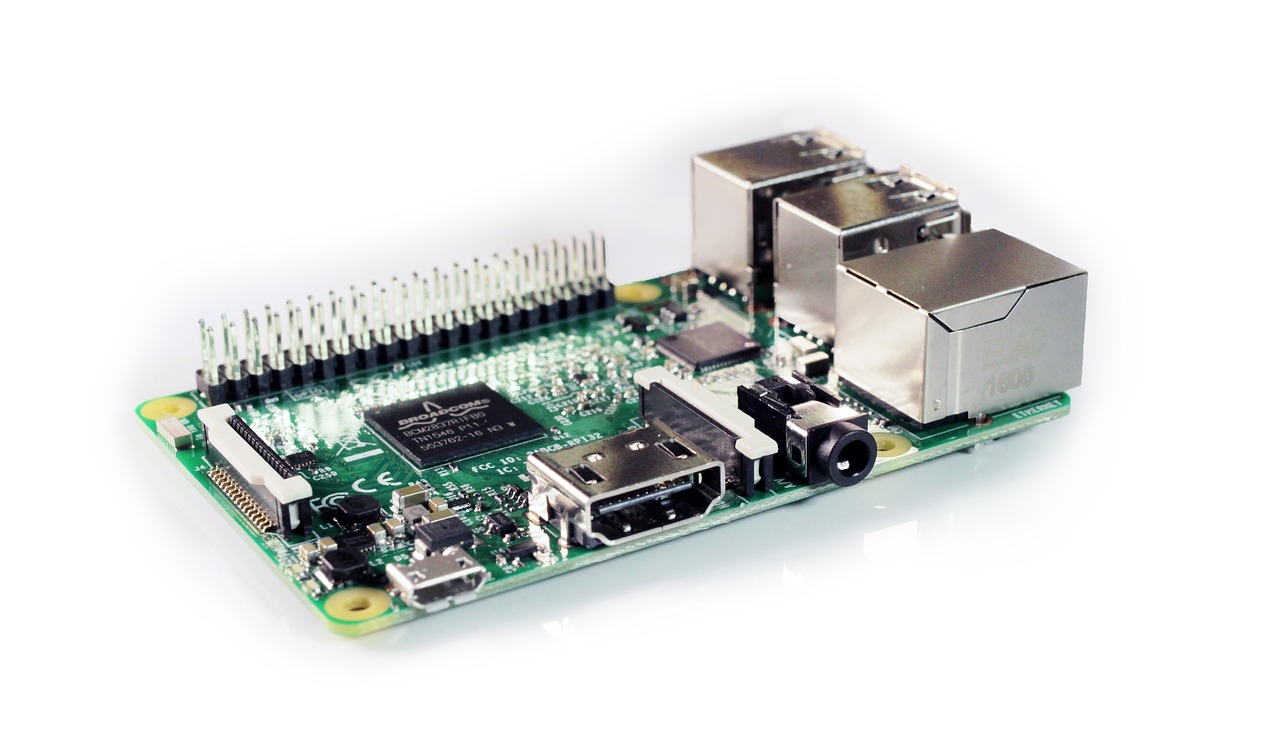
\includegraphics[width=0.8\linewidth]{bilder/raspberry-pi}
	\caption[Raspberry Pi 3 - Einplantinencomputer]{Der Raspberry Pi 3 - Einplantinencomputer \cite{PixaPi2016}}
	\label{fig:server_diagram}
\end{figure}


\subsection{Zielsetzung}\label{sec:zielsetzung}
Seit dem Erfolgskurs des Web 2.0\footnote{Web 2.0 ist ein Schlagwort, das für eine Reihe interaktiver und kollaborativer Elemente des Internets, speziell des World Wide Webs, verwendet wird. Dabei konsumiert der Nutzer nicht nur den Inhalt, er stellt als Prosument selbst Inhalte zur Verfügung. - Wikipedia.org} in den frühen 2000er Jahren, zeichnet sich zunehmend der Trend des Software-as-a-Service Geschäftsmodells ab. Dies beschreibt die Bereitstellung von Software im Internet oder durch ein lokal laufenden Servers, ohne dass Benutzende die Software selbst noch lokal installiert haben müssen. Im Jahr 2015 setzten bereits über drei Viertel von 102 befragten Unternehmen Software dieser Form aktiv im Geschäft ein\cite{TecArt-GmbH2019:online}. Viele Arten von Software können  mittlerweile in einer im Webbrowser lauffähigen Alternative substituiert werden. Ein populäres Beispiel ist die Office-Suite Google Docs der Firma Google inc. Hier lassen sich Textverarbeitung, Tabellenkalkulation und das erstellen von Präsentationen ohne Installation und direkt im Webbrowser des Benutzenden ausführen. Ein anderes Beispiel ist die Web-Software Photopea welche ebenfalls komplett im Web-Browser ausgeführt wird und dem nur lokal installiert ausführbaren quasi Industriestandard Bildbearbeitungsprogramm Photoshop der Firma Adobe inc. sehr nahe kommt. Im Vergleich zu lokal installierter Software ist die Bereitstellung von Web-Software einfacher, da solange ein moderner Webbrowser lauffähig ist, das Betriebssystem des Client-Computers zu vernachlässigen ist. Ebenso stellt potente Hardware keine zwingende Voraussetzungen, da etwaige rechenintensive Aufgaben auf der Serverseite getätigt werden können oder hier eine Balance zwischen Client und Server angestrebt werden kann. \\ 
% Das da oben noch Teil der Problemstellung?
%Hier jetzt Web Trend noch erwähnen!
Ein Raspberry Pi Einplantinencomputer bietet bereits genügend Leistung für Webtechnologien und ein günstigen Anschaffungspreis. Auch besitzen bereits 67\% der 10-11 jährigen Jugendlichen ein Smartphone \cite{Statista2017:online} welches ebenfalls genug Leistung für Webanwendungen aufweisen. \\ \\ Eine Softwarelösung zur Unterstützung von interaktiven Unterrichtsmethoden, welche auf Webtechnologien basiert, könnte den Rahmen der im Digitalpakt Schule fließenden Gelder optimierter ausschöpfen und Schulen finanzielle Flexibilität einräumen. 
\\ \\
Diese Arbeit wird sich der Thematik von pädagogischen digitalen Konzepten und Varianten von interaktiven Unterrichtsmethoden nur im Rahmen der Softwareentwicklung widmen und ihre forschungsrelevante Tiefe nicht gänzlich erfassen, da dies den Rahmen der Zielsetzung überschreiten würde.

%wichtigste Quellen hier noch nennen un
\newpage

\subsection{Aufbau der Arbeit}
Im Anschluss an dieses Kapitel werden \hyperref[sec:grundlagen]{\textbf{Grundlagen}} erörtert. Dies umfasst die Themengebiete Digitalisierung an Schulen und einen Überblick über Webtechnologie. Ersteres ist für den späteren potentiellen Einsatz der Software maßgebend, letzteres bildet das technologische Fundament, welches die Implementierung erst möglich macht. Anschließend wird in Kapitel \hyperref[sec:analyse]{\textbf{Analyse}} ein Vergleich zwischen existierenden kommerziellen und nicht-kommerziellen Plattformen gezogen. Darauf aufbauend folgt eine Anforderungs- und Systembeschreibung. Im darauffolgenden Kapitel \hyperref[sec:konzept]{ \textbf{Konzept}} wird ebendieses erörtert und darauffolgend der Prozess der \hyperref[sec:implementierung]{\textbf{Implementierung}} beschrieben. In einer folgenden \hyperref[sec:auswertung]{\textbf{Auswertung}} werden die Ergebnisse mit den geplanten Zielen verglichen und ein Fazit gezogen. Schlussendlich wird im letzten Abschnitt ein \hyperref[sec:ausblick]{\textbf{Ausblick}} formuliert, welcher die Zukunft des Projekts betrifft. 
   

\newpage

\section{Grundlagen}\label{sec:grundlagen}
Dieses Kapitel soll einen grundlegenden Überblick über die zwei wichtigsten Themen dieser Arbeit bieten, Dclearigitalisierung an Schulen und der damit verbundene Einsatz von digitalen Unterrichtsmethodiken
\subsection{Digitalisierung an Schulen}
\subsubsection{Digitale Technik im Unterricht}\label{sec:technikunterricht}
\subsubsection{Ausblick Interaktive Unterrichtsmethoden}\label{sec:interaktiveunterr}
\subsubsection{Datenschutz an Schulen}\label{sec:datenschutz}

\subsection{Überblick Webtechnologie}\label{sec:webbasedsoftware}
% Hier auf PDF Technische Anforderungen verweisen (Footnote?) da sehr ausführlich und gut
% Anfang Geschichtlich
Diese Sektion soll einen grundlegenden über im Kontext dieser Arbeit wichtigen Begrifflichkeiten bieten. Die folgenden Untersektion 2.2.1 ff. werden die Thematiken nur grob umreißen, da eine detaillierte Betrachtung der genannten Begriffe den Rahmen dieser Arbeit weit überschreiten würde. 

\subsubsection{Intranet und Internet}\label{sec:intranetundinternet}
% Detailgrad so sinnvoll?
% Unterschied und Gemeinsamkeit klar machen
% Hier kommunikation erklären! Protokolle und OSI schicht!
Einfach ausgedrückt, ist das Internet ein Netzwerk von Computern, welche weltweit miteinander vernetzt sind. Seine Anfänge lassen sich auf das Ende der 1960er in den USA datieren, als die DARPA (Defense Advanced Research Projects Agency) eine weltweite Verknüpfung von Datennetzen anstrebte. Das hier draus resultierende ARPANET (Advanced Research Projects) kann als Ursprung angesehen werden. Dabei beschreibt der Begriff Internet streng genommen ein 'interconnected network', also ein international vernetztes Netzwerk, ohne dabei die Hardware- und Netzwerktechnologie genauer zu beschreiben \cite{safran2011webtechnologien:article}.  \\ 
Der wohl populärste Anwendung des Internets ist das World Wide Web, welche gegen das Jahr 1989 von einer Forschungsgruppe rund um Sir Tim Berners-Lee ins Leben gerufen wurde und heute oftmals als Synonym für das gesamte Internet sprachlich genutzt wird. \\ 

In unser heutigen globalisierten Welt lässt sich das Internet mitsamt World Wide Web nicht mehr wegdenken und ist ein integraler Bestandteil der Informationskultur. 
 \\ \\
 Das Intranet beschreibt analog dazu ein lokal abgeschlossenes Netzwerk von Computern, bspw. innerhalb eines Unternehmens. Dabei endet ein Intranet klar an seinen Grenzen und ein Gateway fungiert als Übergabepunkt ins Internet. Die Vernetzung der Endgeräte erfolgt kabelgebunden (LAN) oder kabellos (WLAN). Die Kommunikationsgeschwindigkeit innerhalb eines Intranets sind i.d.R. deutlich höher als im Internet, da Daten nicht erst nach außen an einen Internet Service Provider übermittelt werden müssen. Ein Intranet funktioniert unabhängig vom öffentlichem Internet (erhöhte Ausfallsicherheit), ist nicht öffentlich zugänglich und bietet oft andere oder zusätzliche Funktionen. \cite{Intranet62:online}. 
 
 \subsubsection{Client-Server Modell}\label{sec:clientservermodell}
 Das Client-Server Modell beschreibt das Prinzip der Kommunikation zwischen zwei Teilnehmer innerhalb eines Netzwerks. Grundlegend unterscheidet das Modell hierbei zwischen einer Anbieterseite (Server) und einer Benutzerseite (Client). Der Client betreibt auf seinem Endgerät (Computer, Smartphone, etc.) eine Clientsoftware mit der die Verbindung zum Server aufgebaut wird. Im Fall des WWW (siehe \ref{sec:www}) ist dies in den meisten Anwendungsszenarien ein Webbrowser. Der Client fordert dabei eine Resource an, welche auf dem Server vorliegt oder dort speziell für die Anfrage des Clients generiert wird (siehe auch Sektion \ref{sec:webanwenservices}). Das Client-Server Modell sieht vor, dass immer der Client die Verbindung aufbaut, nie andersherum \cite{ElektronikKompendium.de:online}. Die Anfrage des Clients wird Request genannt, die Antwort des Servers Response oder Reply, welche bei ausreichender Berechtigung des Clients auch Daten enthält. 
 Server-Computer sollen rund um die Uhr erreichbar sein, während Client-Endgeräte auch abgeschaltet werden können, ohne die Integrität des Netzwerks zu beeinflussen. 
  % Vergleich zu anderen Modellen?
 
\subsubsection{Kommunikation}\label{sec:kommunikation}
Die Kommunikation im Internet und Intranet erfolgt über Protokolle. 
Ein Protokoll kann als ein Satz von Kommunikationsregelvorschriften verstanden werden \cite{safran2011webtechnologien:article}, welche den Netzwerkverkehr auf unterschiedlichen Schichten reglementieren. 
Diese Schichten werden im OSI-Modell (Open System Interconnection) der ISO (International Standardization Organisation), der internationalen Standardisierungsorganisation beschrieben. (Siehe Tabelle) %HIER TABELLE!
\\ 
Das OSI-Modell ist dabei in sieben Schichten eingeteilt, während die Erste als physikalische Schicht definiert ist und die Siebte als Anwendungsschicht. Protokolle sind dabei jeweils nur über Protokolle benachbarter Schichten in Kenntnis gesetzt. Das OSI-Modell lässt sich grob in anwendungsorientierte Schichten (1 bis 4) und transportorientierte Schichten (5 bis 7) unterteilen. Die im Rahmen dieser Arbeit genutzten Webtechnologien nutzen kommunikativ nur anwendungsorientierte Schichten des ISO-OSI Modells.



% Begriff Internet
\subsubsection{World Wide Web}\label{sec:www}
Das World Wide Web (WWW) ist die wohl populärste Anwendung des Internets \cite{safran2011webtechnologien:article} und wird oftmals fälschlicherweise als Synonym für das gesamte Internet genannt. Das WWW ist eine Sammlung von verteilten Dokumenten, welche sich gegenseitig über sog. Hyperlinks referenzieren und von Web-Servern zur Verfügung gestellt werden. Auf der Client Seite (siehe \ref{sec:clientservermodell}) stellt der Web-Browser die wichtigste Software da. Mit ihr werden Web Server angesprochen (Request) und Antworten (Response) für den Nutzenden dargestellt. Die wichtigsten sprachlichen Komponenten des WWW sind: \\ 
\begin{itemize}
	\item HTML: Hypertext Markup Language - eine reine Beschreibungssprache, welche Hypertext Dokumente durch Tags codiert. 
	\item CSS: Cascading Style Sheet - Eine Stylesheet Sprache, welche das äußere Erscheinungsbild von Hypertext Dokumenten beschreibt
	\item JS: JavaScript: Eine Skriptsprache, welche u.A. Interaktion sowie Dynamik hinzufügt und clientseitig interpretiert wird. 
\end{itemize}
Die Techniken des WWW können auch lokal im Intranet genutzt werden. 
Das zur Verständigung zwischen Client und Server genutzte Protokoll (siehe \ref{sec:kommunikation})ist das Hypertext Transfer Protocol (HTTP) bzw. in verschlüsselter Form Hypertext Transfer Protocol Secure, da eine Übermittlung im Klartext nicht immer wünschenswert ist. HTTP/HTTPS ist ein Zustandsloses Protokoll, das bedeutet dass jede Anfrage unabhängig voneinander geschieht und betrachtet wird. Dies und die Tatsache, dass jede Anfrage von der Client-Seite aus gestartet werden muss (siehe \ref{sec:clientservermodell}), stellen oftmals Hürden für die Entwicklung von Webanwendungen und Webservices da. Techniken wie Cookies und Sessions, sowie das wiederholte Abfragen von aktualisierten Daten seitens des Clients wirken hier entgegen. Cookies stellen persistent gespeicherte Daten auf der Client-Seite da, mit deren Hilfe der Webserver einen Client eindeutig zuordnen kann. Bei einer Session sendet der Client bei jeder Anfrage eine eindeutige ID an den Server. Im Normalfall endet eine Session beim Beenden des Webbrowser, während Cookie-Dateien eine längere Lebensdauer besitzen.      
%
\subsubsection{Webanwendungen und Webservices}\label{sec:webanwenservices}
Im Laufe der Entwicklung des WWW (\ref{sec:www}) stieg der Anspruch vom reinen Anbieten statischer Dokumenten in Richtung dynamischer Inhalte, welche einer Programmlogik folgend von einem Webserver für jede Anfrage generiert werden. Webanwendungen sind Computerprogramme, welche auf einem Webserver ausgeführt werden und den Webbrowser des Clients als Schnittstelle nutzen \cite{safran2011webtechnologien:article}. Dies bietet den großen Vorteil, dass etwaige Anpassungen von Programmlogik nur serverseitig erfolgen müssen und jeder Client mit Webbrowser als Benutzerschnittstelle ausreicht. \\ \\
Webservices sind eine spezialisierte Art von Webanwendung. Die Fokus hier liegt auf das bereitstellen von Daten für andere Applikationen, welche die gewonnen Daten selbst auswerten und dem Nutzenden bereitstellen. Dies geschieht i.d.R. über eine einheitlich beschriebene Schnittstelle (API - Application Programming Interface), über welche fremde Applikationen angefragte Daten abrufen können. Der Austausch der Daten erfolgt hier meist über Formate wie JSON (JavaScript Object Notation) oder XML (Extensible Markup Language), da Aussehen und Lesbarkeit der Daten irrelevant sind und somit eine Ausgabe in HTML nicht von Nöten ist. \\
Bei der Implementierung eines Webservices bieten sich folgende zwei technologische Arten der Umsetzung an: \\ \\
\textbf{SOAP/WSDL}: Hier werden Nachrichten über das Simple Object Access Protocoll ausgetauscht (SOAP) und deren Beschreibung über die Web Services Description Language (WSDL) definiert. Anfrage- und Antwortformat der Daten ist XML (Extensible Markup Language), eine Auszeichnungssprache, welche HTML sehr ähnelt aber deutlich allgemeiner ist. XML kann als mehr als Regelwerk verstanden werden, mitdessen Hilfe Entwickler ihre eigene hierarische Beschreibung einer Datenstruktur vornehmen können. XML und HTML leiten sich bei der von der SGML (Standard Generalized Markup Language) ab, welches ihre Ähnlichkeit zusätzlich herleitet \cite{XMLHTMLU88:online}. \\

 
\textbf{REST}: (Representational State Tranfer) Hier kann jede einzelne Funktion des Webservices über eine jeweils zugeordnete URL abgerufen (Uniform Resource Locator) werden, umgangssprachlich als Webadresse bekannt. Das WWW selbst kann als REST-Webservice verstanden werden \cite{Bayer2002:online}. \\ 

\subsection{Websockets}\label{sec:websockets}
Bezugnehmend auf die Problematik, welche durch die Kommunikationsstrategie über das http-Protokoll entsteht (siehe Sektion \ref{sec:www}), wirken Websockets dieser entgegen. Als Kommunikationskanal verknüpft ein Websocket Server und Client. Zwar muss die Kommunikation zunächst über den Client initiiert werden, bleibt dann jedoch bestehen und der Server kann diese nutzen um aktiv neue Daten zu emittieren. Ein Nachteil ist jedoch, dass im Gegensatz zum http-Protokoll hier auch Daten hin- und hergeschickt werden, wenn dies eventuell nicht gewünscht ist \cite{neumann2015entwicklung}, was insbesondere bei mobilen Applikationen kritisch sein kann. 

\subsection{Webapplikationsentwicklung}\label{sec:softwareentwicklung}
Dieses Kapitel soll den wesentlicheren Bestandteil dieser Arbeit grundlegend beleuchten, der Entwicklung von Webapplikationen.
Webanwendungen und Webservices können unter diesem Begriff zusammengefasst werden.
 \\ 
\subsubsection{Web-Application-Frameworks} \label{sec:wafs}
Bei der Entwicklung von Webapplikationen wird oftmals auf Frameworks (z.Dt. Rahmengerüste), spezifischer Web-Application-Framework (WAF) zurückgegriffen. 
Ein WAF bezeichnet damit ein Programmgrundgerüst, welches als Grundlage zum Einsatz kommt \cite{Ionis2019:online}. Dies erleichtert die Entwicklung ungemein, da auf bereits vorgefertigte Ansätze und Programmbausteine zugegriffen werden kann und diese nicht selbst von Hand implementiert werden müssen. Diese WAFs reflektieren zumeist auch eine Modelle und Prinzipien, welche, falls dem Entwickelnden bekannt, den Einstieg erleichtern. 
Ein für Frameworks bekanntes Paradigma stellt das Umsetzungsparadigma \\
\textbf{Inversion of Control} (IoC), z.Dt. Umkehrung der Steuerung da, welches u.a. auch in der objektorientieren Programmierung Anwendung findet.
Hierbei wird eine Funktion/Unterprogramm bei der Hauptprogrammbibliothek registriert und von dieser zu einem späteren Zeitpunkt aufgerufen. Dies ist umgangssprachlich auch als 'Hollywood'-Prinzip bekannt ('Don't call us! We call you' z.Dt. 'Ruf nicht uns an! Wir rufen dich an!'). Das Framework behält also die Programmflusssteuerung bei. 
  Ein Nachteil, der durch dein Einsatz von einem WAF bedingt ist, stellt die Einschränkung der Freiheit während des Implementierungsprozesses da, dieser wird jedoch billigend in Kauf genommen, da sich ein Reduktion des Zeit- und Kostenaufwands erhofft wird. Die Wahl des richtigen WAF ist ein wichtiger Entschcheidungsprozess, bei dem mehrere Faktoren beachtet werden müssen, wie z.B. benötigte Einarbeitungszeit und Lizenzen.

\subsubsection{Serverseitiger Ansatz}\label{sec:serverseitgeransatz}
Anknüpfend an Sektion \ref{sec:webanwenservices}, sind Webapplikationen Software, welche Serverseitig ausgeführt werden, wobei der Webbrowser eines Nutzenden als Benutzerschnittstelle dient. Eine Webapplikation kann jedoch auch clientseitig implementiert werden, wie in Sektion \ref{sec:clientseitigeransatz} beschrieben. \\ \\
Serverseitige Webapplikationen verfolgen oftmals den Multi-Page Ansatz, das heiß pro Anfrage (Request) wird eine anderes Dokument dem Client (Webbrowser) übergeben. Wichtige Programmiersprachen für den Ansatz sind php, Ruby, Python, Java und auch JavaScript, was vorher zunächst nur auf der Clientseite zur Anwendung kam. \\
Die \textbf{Model - View - Controller} Architektur (MVC) ist vorherrschende Architektur, auf welche sich der Großteil der serverseitigen WAFs stützen.
Hierbei wird die Programmlogik klar in drei große Bestandteile unterteilt: \\
\textbf{Model}: Das Model oder z. Dt. Modell beschreibt eine Datenstruktur an sich. In einem Webshop wären dies z.B. die Produkte und deren Eigenschaften wie ID, Name, Preis usw. \\
\textbf{View}: Diese beschreibt die reine Ansicht eines Dokuments. In einem Webshop wäre dies z.B. die Detailseite eines Produkts. Dabei sollte so wenig wie nötig Logik selbst im Code der View vorkommen. \\
\textbf{Controller}: Der Controller dient als Bindeglied zwischen Model und View. Er handelt ankommende Requests (Anfragen) ab und übergibt der View aus dem Modell die notwendigen Daten. \\ 
Neben der MVC Architektur existieren weitere, andere Architekturen und Ableitungen der MVC Architektur, wie z.B. der im Django WAF genutzten Model - View - Presenter Architektur. \\
Es folgt eine Tabelle, die einen groben Überblick über bekannte WAFs, welche den serverseitigen Multi-Page Ansatz verfolgen \cite{TopWebDe0:online}. 

\begin{table}[H]
	\centering
	\caption{Überblick serverseitiger Web-Application-Frameworks}
	\label{tab:spektrometer}
	\begin{tabular}{lcc}
		\textbf{Name} & \textbf{Sprache} & \textbf{Architektur}   \\ 
		\hline 
		Symfony & php & Model - View - Controller \\
		Laravel	& php & Model - View - Controller  \\ 
		Phalcon	& php & Model - View - Controller   \\ 
		Codeigniter & php & Model - View - Controller \\
		Django & Python & Model - View - Presenter \\		
		Ruby on Rails & Ruby & Model - View - Controller \\
		\hline 
	\end{tabular} 
\end{table}


Aus der Tabelle lässt sich eine starke Popularität der Programmiersprache php ableiten und deren auf dieser Sprache basierenden WAFs. Die Tabelle stellt keinen Anspruch auf Vollständigkeit, da noch unzählig viele andere serverseitige WAFs existieren, die den Rahmen der Tabelle überschreiten würden. Ebenso wurde das WAF ExpressJS, welches auf der serverseitigen Plattform NodeJS basiert, bewusst nicht mit in die Tabelle aufgenommen, da dies ein Sonderfall darstellt. Diese Thematik wird in Kapitel \ref{sec:konzept} ausführlich behandelt. 
%Hier über NodeJS und PHP quatschen!
\subsubsection{Clientseitiger Ansatz}\label{sec:clientseitigeransatz}
 Das Programmiermodell des WWW, welches durch die Architektur des Hypertext Transfer Protocol (HTTP) geprägt ist, wird bei der Entwicklung von Webapplikationen übernommen. Dies sieht eine Anfrage immer seitens des Clients vor (siehe auch Sektion \ref{sec:www}). Dies schränkt das Ausmaß von Interaktion und generieren von dynamisch ladenden Webseiten ein. 
 Der clientseitige Ansatz der Webapplikationsentwicklung kommt meistens bei sog. Single-Page Applikationen zutrage. Hierbei wird o.g. Problem damit umgangen, indem bei Aufruf einer Internetseite die gesamte HTML Benutzeroberfläche inklusive Programmlogik in Form von JavaScript Code als Ganzes an die Client übergeben wird. Dies bietet den großen Vorteil, dass die Logik nun auf dem Client ausgeführt wird und dieser dynamisch Daten nachladen bzw. Anfragen kann. Oftmals ändert sich auf einer Single-Page Applikation die Webadresse in der Adresszeile des Browsers nicht. Die ganze Applikation läuft also auf einer einzelnen Website ab, die sich dynamisch ändert. Dieses dynamische Nachladen von Inhalten wird \textbf{AJAX} - Asynchronous JavaScript and XML genannt.  Die einzig nativ unterstützte Programmiersprache seitens der Webbrowser ist JavaScript und daher vorherrschend \cite{safran2011webtechnologien:article}.
 Jeder moderne Webbrowser hat einen JavaScript Interpreter integriert. Über Plugins können zwar auch andere Sprachen genutzt werden, in Form von Java-Applets (Programmiersprache dort Java )oder das früher sehr populäre Flash des Unternehmen Adobe, welches ActionScript als Programmiersprache nutzt. Beides gilt aber Stand 2019 als veraltet und der Einsatz derartigen Technologien wird nicht empfohlen. %Nachweis nötig?
Es gibt sehr viele JavaScript WAFs und Bibliotheken, zu den bekanntesten zählen: \\ \\ 
% hier noch bisschen mehr vielleicht
 \textbf{Angular} ist ein clientseitiges JavaScript WAF, entwickelt und bereitgestellt von dem Unternehmen Google. Es hat vergleichsweise eine steile Lernkurve und setzt etwas Einarbeitungszeit voraus. \\ 
 \textbf{React} ist streng genommen kein WAF, sondern lediglich eine JavaScript Bibliothek. Es bietet aber über Erweiterungen die Möglichkeit, wie ein WAF genutzt zu werden, was seine Flexibilität noch erhöht. Entwickelt und Betrieben wird React von der Firma Facebook inc. \\
 \textbf{Vue} ist ein clientseitiges JavaScript WAF, ursprünglich entwickelt von Evan You. Es gilt als einfacher zu erlenen als Angular und ist sehr flexibel. \\
 
 
 Das Entwickeln von clientzentrischen JavaScript Anwendungen ist mittlerweile so fortgeschritten, dass oftmals beim Nutzenden ein Gefühl entsteht, es würde ein lokal installiertes Programm ausgeführt werden. Populäre Beispiele wäre das in Kapitel \ref{sec:zielsetzung} erwähnte Google Docs, welches eine voll umfassende Textverarbeitungslösung im Browser bietet. Derartige Applikationen werden Rich Internet Application (RIA) genannt.
 

%Hier vor allem über Javascript quatschen!
\subsubsection{Hardware Anforderungen}\label{sec:hardware}
Auf der \textbf{Serverseite} ist der Anspruch an die Hardware sehr abhängig vom gewünschten Anwendungsfall und benötigter Skalierbarkeit. Das beliebte Server Linux Derivat Debian benötigt bspw. mindestens 128 Megabyte Ram-Speicher und 2 Gigabyte Festplattenspeicher. Es ist aber durchaus möglich mit noch sehr viel weniger potenter Hardware ein Server zu betreiben \cite{dpakt2019:online}. 
\subsubsection{Vergleich zu anderen Entwicklungsansätzen}\label{sec:vorundnachteileweb}
Der klassische Ansatz der Software Entwicklung wäre das implementieren eine Desktop-Anwendung, welche lokal
auf dem Computer des Anwendenden installiert wird. Typischerweise wird die Software programmiert und anschließend von einem Compiler in Maschinencode übersetzt bzw. von einer Laufzeitumgebung zur Ausführung interpretiert. Die Software wird also normalerweise auf dem Computer installiert und an die Gegebenheiten des Betriebssystems angepasst. Dies hat den Vorteil bei Bedarf sehr hardwarenah und performant entwickeln zu können, was durch das vorherige kompilieren des Codes in Maschinencode begünstigt wird. Nachteilig ist es jedoch, dass die Software zunächst überhaupt installiert werden muss. 

\begin{table}[H]
	\centering
	\caption{Webapplikationsentwicklung im Vergleich \cite{TecArt-GmbH2019:online}}
	\label{tab:spektrometer}
	\begin{tabular}{l | p{5cm}|  p{5cm}}
		\textbf{Kriterium} & \textbf{Webapplikation} & \textbf{Desktopapplikation}   \\ 
		\hline 
		Struktur & Modularer Aufbau & Meist als Gesamtpaket vertrieben \\
		\hline 
		Verfügbarkeit & Weltweit dank Internet, lokal eingeschränkt möglich & Nur bei lokaler Installation verfügbar \\ 
		\hline 
		Installation	& Nicht erforderlich & Erforderlich   \\ 
		Speicher & Kein Zusätzlicher Speicher benöntigt & Installation benötigt Speicherplatz \\
		\hline 
		Updates & Live-Aktualisierung möglich & Teil- oder Neuinstallation notwendig \\		
		\hline 
		Teamarbeit & Zeitgleiches und schnelleres Arbeiten leicht möglich & Teamarbeit nur über Synchronisation möglich \\
		\hline 
	\end{tabular} 
\end{table}


\newpage

\section{Konzept}\label{sec:konzept}
\newpage

\section{Implementierung}\label{sec:implementierung}
\newpage

\section{Erprobung}\label{sec:erprobung}
\newpage

\section{Fazit}\label{sec:fazit}
\newpage

\section{Ausblick}\label{sec:ausblick}
\newpage


%\fancyhead[L]{\textsl{\small \leftmark}}
%\input{sections/07Zusammenfassung.tex}%\newpage
%\input{sections/08Ausblick.tex}\newpage

%\addcontentsline{toc}{section}{Literaturverzeichnis}
%\printbibliography[nottype=online, title={Literaturverzeichnis}]
%\printbibliography[type=online,title={Online - Bildquellen}]\newpage

\printbibliography[title={Literaturverzeichnis}]
\newpage


\addcontentsline{toc}{section}{Abbildungsverzeichnis}
\listoffigures\newpage
\addcontentsline{toc}{section}{Tabellenverzeichnis}
\listoftables

%\clearpage%\vspace*{-3cm}
%\newpage

\addcontentsline{toc}{part}{Anhang}

\fancyhead[L]{\textsl{\small \leftmark \hspace{0.8cm}\rightmark}}

%\appendix % Für Anhänge
%\input{anhang/Zemente}
%\input{anhang/Nachmessung_Zemente}



\end{document}